
\documentclass{article}
\usepackage[utf8]{inputenc}
\usepackage{amsmath}
\usepackage{amsfonts}
\usepackage{amssymb}
\usepackage{graphicx}
\usepackage{float}

% Configuración del título

    
\title{Informe de Análisis Exploratorio de \texttt{mtcars}}
\author{
  Melani Forsythe Matos \\
  Daniela Guerrero Álvarez \\
  Rubén Martínez Rojas
}
\date{} % Sin fecha para que no aparezca

\begin{document}

\maketitle
\newpage % Inserta una nueva página aquí

El conjunto de datos \texttt{Titanic} es un conjunto clásico que contiene información sobre los pasajeros del Titanic, y se utiliza frecuentemente en análisis de supervivencia. A continuación, se describen las variables incluidas en este conjunto de datos, su significado, tipo de escala, y si son discretas o continuas:

\begin{enumerate}
    \item \textbf{PassengerId}
    
    \begin{itemize}
        \item \textbf{Descripción:} ID único para cada pasajero.
        \item \textbf{Escala:} Cuantitativa Discreta.
        \item \textbf{Significado:} Un identificador numérico para cada pasajero en la base de datos.
    \end{itemize}
    \item \textbf{Class}

    \begin{itemize}
        \item \textbf{Descripción:} Clase del pasajero (1st = Primera, 2nd = Segunda, 3rd = Tercera, Crew = Trabajadores).
        \item \textbf{Escala:} Cualitativa Ordinal.
        \item \textbf{Significado:} Representa la clase socioeconómica del pasajero, con 1 siendo la clase más alta y 3 la más baja, y los trabajadores.
    \end{itemize}

    \item \textbf{Age}
    
    \begin{itemize}
        \item \textbf{Descripción:} Si el pasajero es Adulto o Niño.
        \item \textbf{Escala:} La edad normalmente es una variable cuantitativa, pero en este caso está dividido por grupos etáreos, Adulto y Niño, por tanto se clasifica como Cualitativa Nominal.
        \item \textbf{Significado:} 
    \end{itemize}

    \item \textbf{Survived}

    \begin{itemize}
        \item \textbf{Descripción:} Indicador de supervivencia (No, Sí).
        \item \textbf{Escala:} La variable es Cualitativa Nominal, pero podría convertirse a Cuantitativa Discreta (Binaria), asignándole 1 a Si y 0 a no, o viceversa.
        \item \textbf{Significado:} Indica si el pasajero sobrevivió al hundimiento del Titanic.
    \end{itemize}

    \item \textbf{Sex}
    
    \begin{itemize}
        \item \textbf{Descripción:} Género del pasajero.
        \item \textbf{Escala:} Cualitativa Nominal.
        \item \textbf{Significado:} Indica el sexo del pasajero (hombre o mujer).
    \end{itemize}

    \item \textbf{Freq}
    
    \begin{itemize}
    \item \textbf{Descripción:} Número de pasajeros.
    \item \textbf{Escala:} Cuantitativa Discreta.
    \item \textbf{Significado:} Indica la la \textbf{frecuencia} o el \textbf{número de pasajeros} que caen en cada combinación de las otras variables (\texttt{Class}, \texttt{Sex}, \texttt{Age}, \texttt{Survived}).
    \end{itemize}    
    
    \textbf{Ejemplo:}    
    \begin{itemize}
        \item \textbf{Class}: La clase del pasajero (\texttt{1st}, \texttt{2nd}, \texttt{3rd}, \texttt{Crew}).
        \item \textbf{Sex}: El género del pasajero (\texttt{Male}, \texttt{Female}).
        \item \textbf{Age}: El grupo de edad del pasajero (\texttt{Child}, \texttt{Adult}).
        \item \textbf{Survived}: Si el pasajero sobrevivió o no (\texttt{No}, \texttt{Yes}).
        \item \textbf{Freq}: El número de pasajeros que pertenecen a esa combinación de \texttt{Class}, \texttt{Sex}, \texttt{Age}, y \texttt{Survived}.
    \end{itemize}
    
\end{enumerate}
    Supongamos que tienes la siguiente fila en el dataset:
    
    \begin{center}
    \begin{tabular}{|c|c|c|c|c|}
    \hline
    \textbf{Class} & \textbf{Sex} & \textbf{Age} & \textbf{Survived} & \textbf{Freq} \\
    \hline
    1st & Male & Adult & Yes & 57 \\
    \hline
    \end{tabular}
    \end{center}
    
    Esto significa que \textbf{57 pasajeros adultos de sexo masculino en primera clase sobrevivieron}.
    
    La columna \texttt{Freq} te permite ver cuántas personas están representadas por cada combinación de las otras variables, en lugar de tener una fila separada para cada pasajero individual.
    
    % Imagen 1: Niños Varones Sobrevivientes por Clase
\begin{figure}[H]
    \centering
    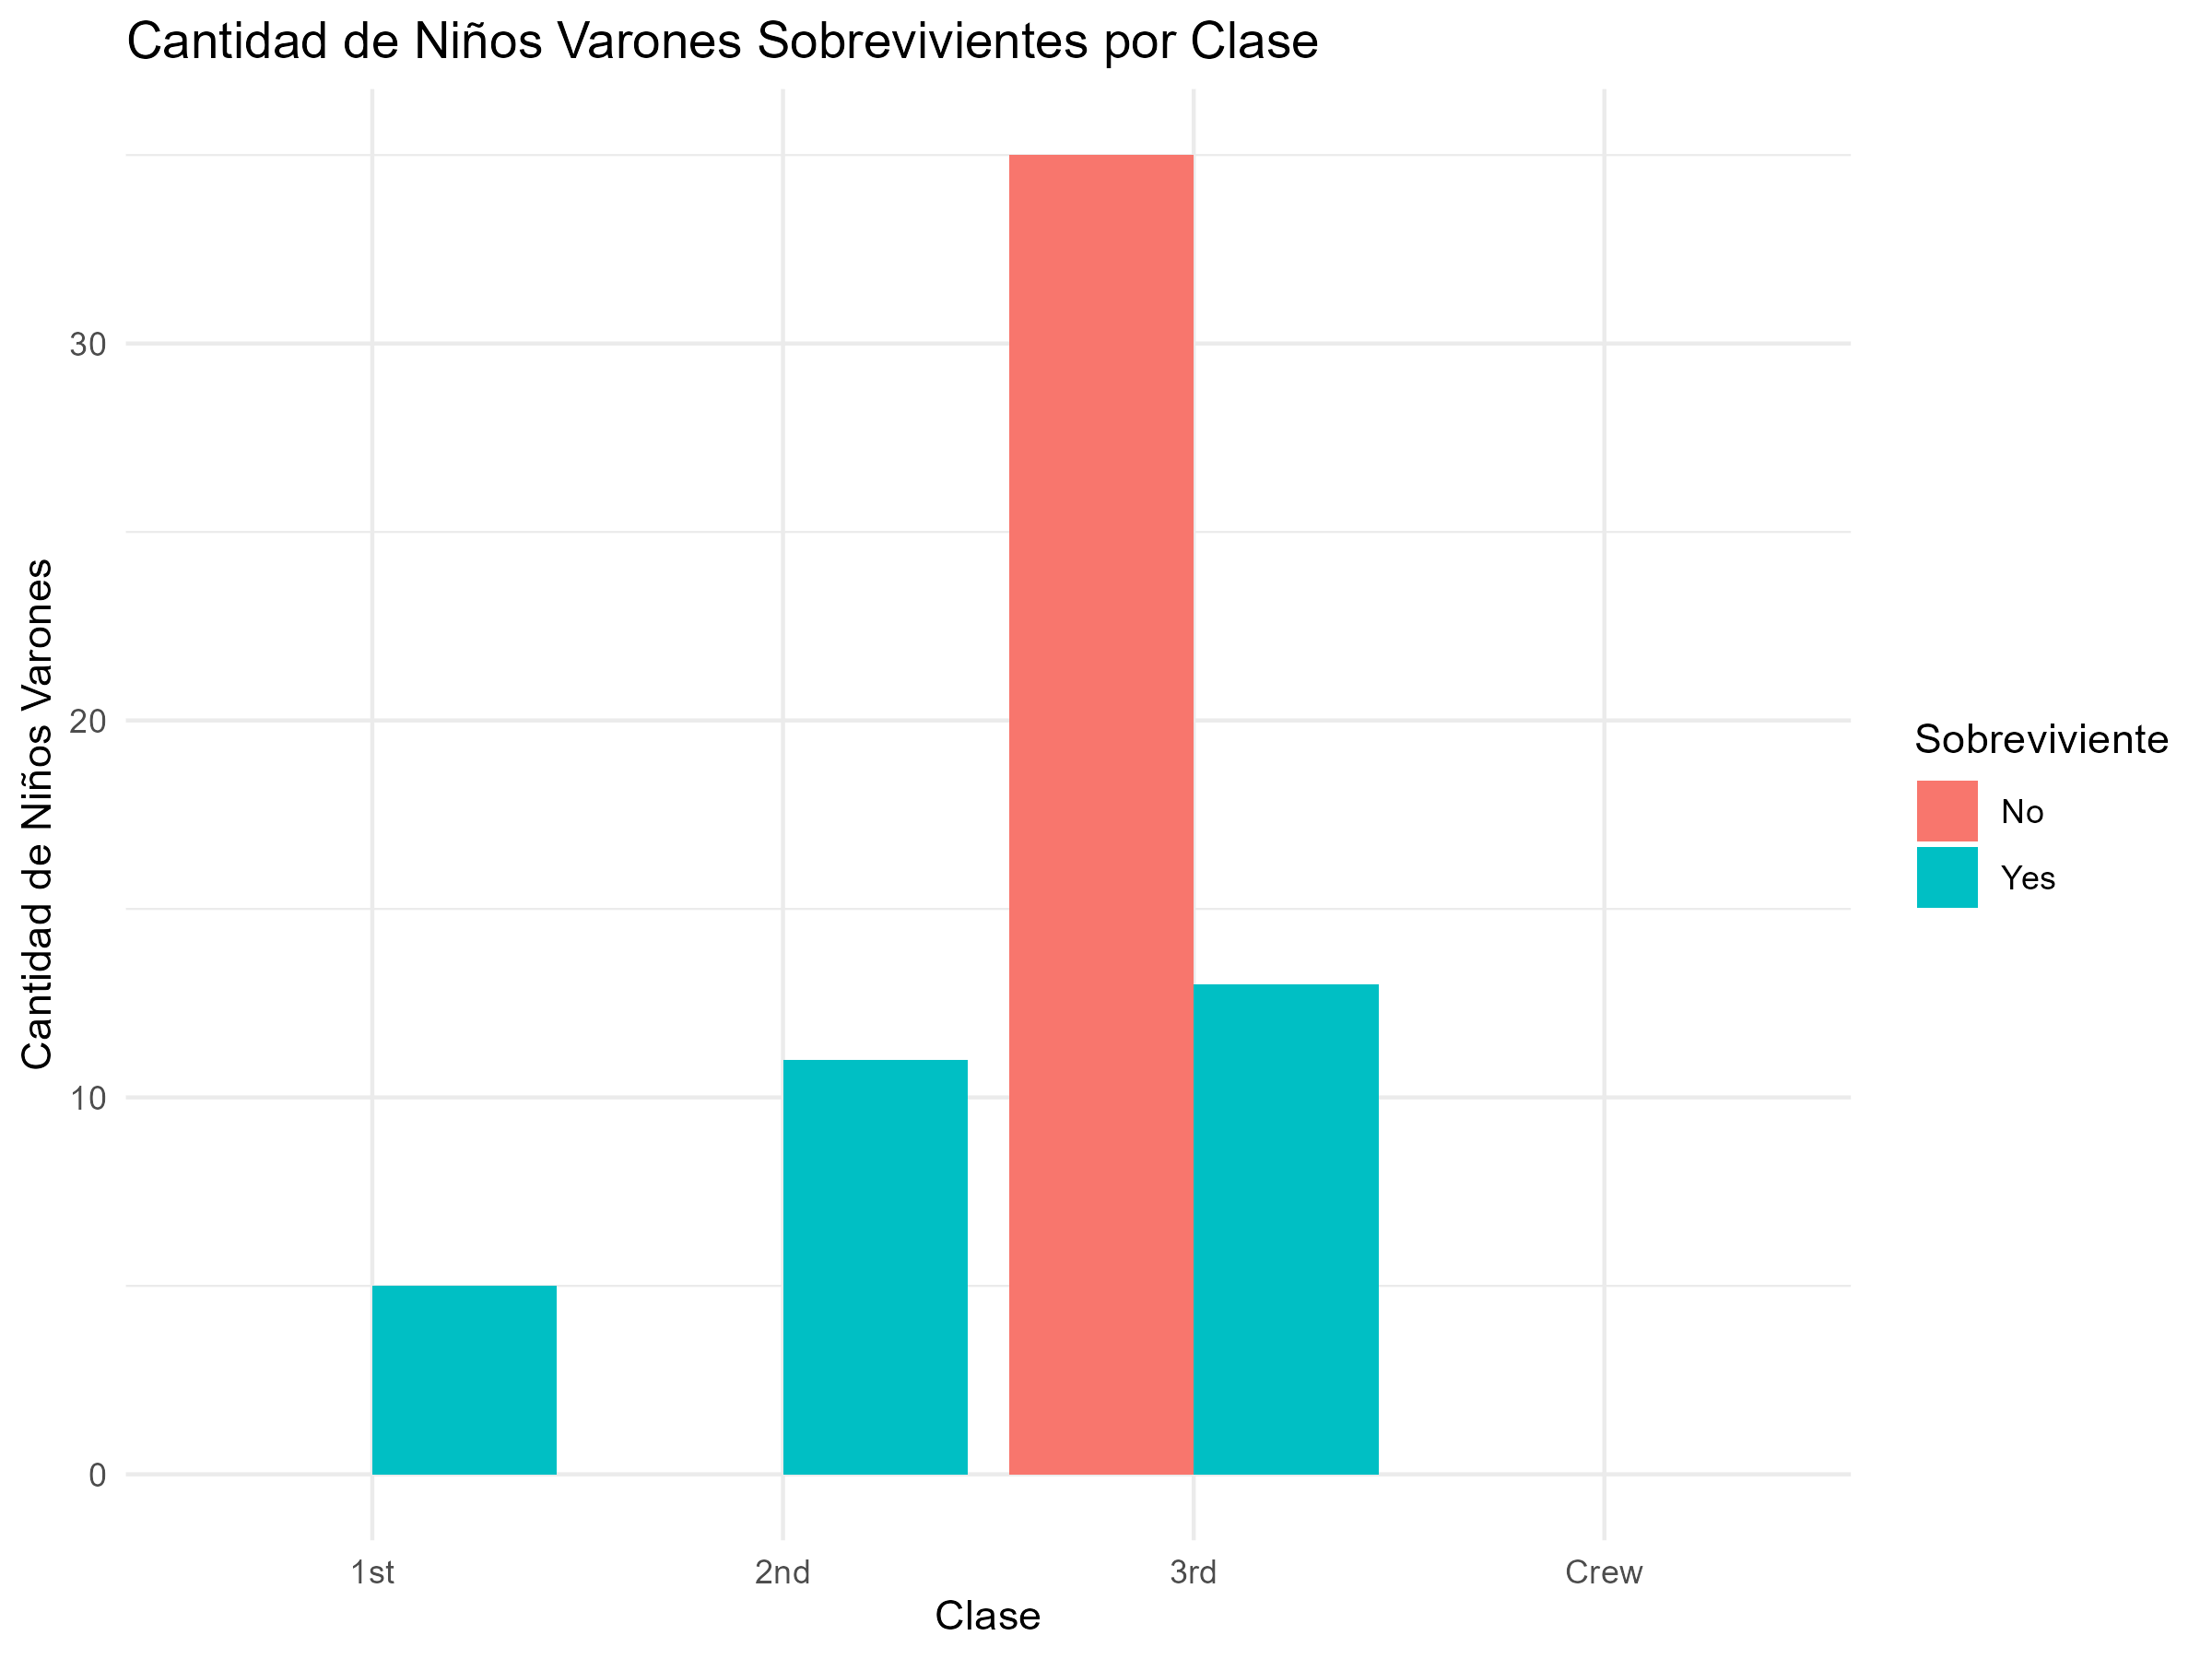
\includegraphics[width=0.8\textwidth]{ninos_varones_sobrevivientes_por_clase.png}
    \caption{Cantidad de Niños Varones Sobrevivientes por Clase}
    \label{fig:ninos_varones_sobrevivientes_por_clase}
\end{figure}

% Texto adicional o explicación aquí

% Imagen 2: Hombres Adultos Sobrevivientes por Clase
\begin{figure}[H]
    \centering
    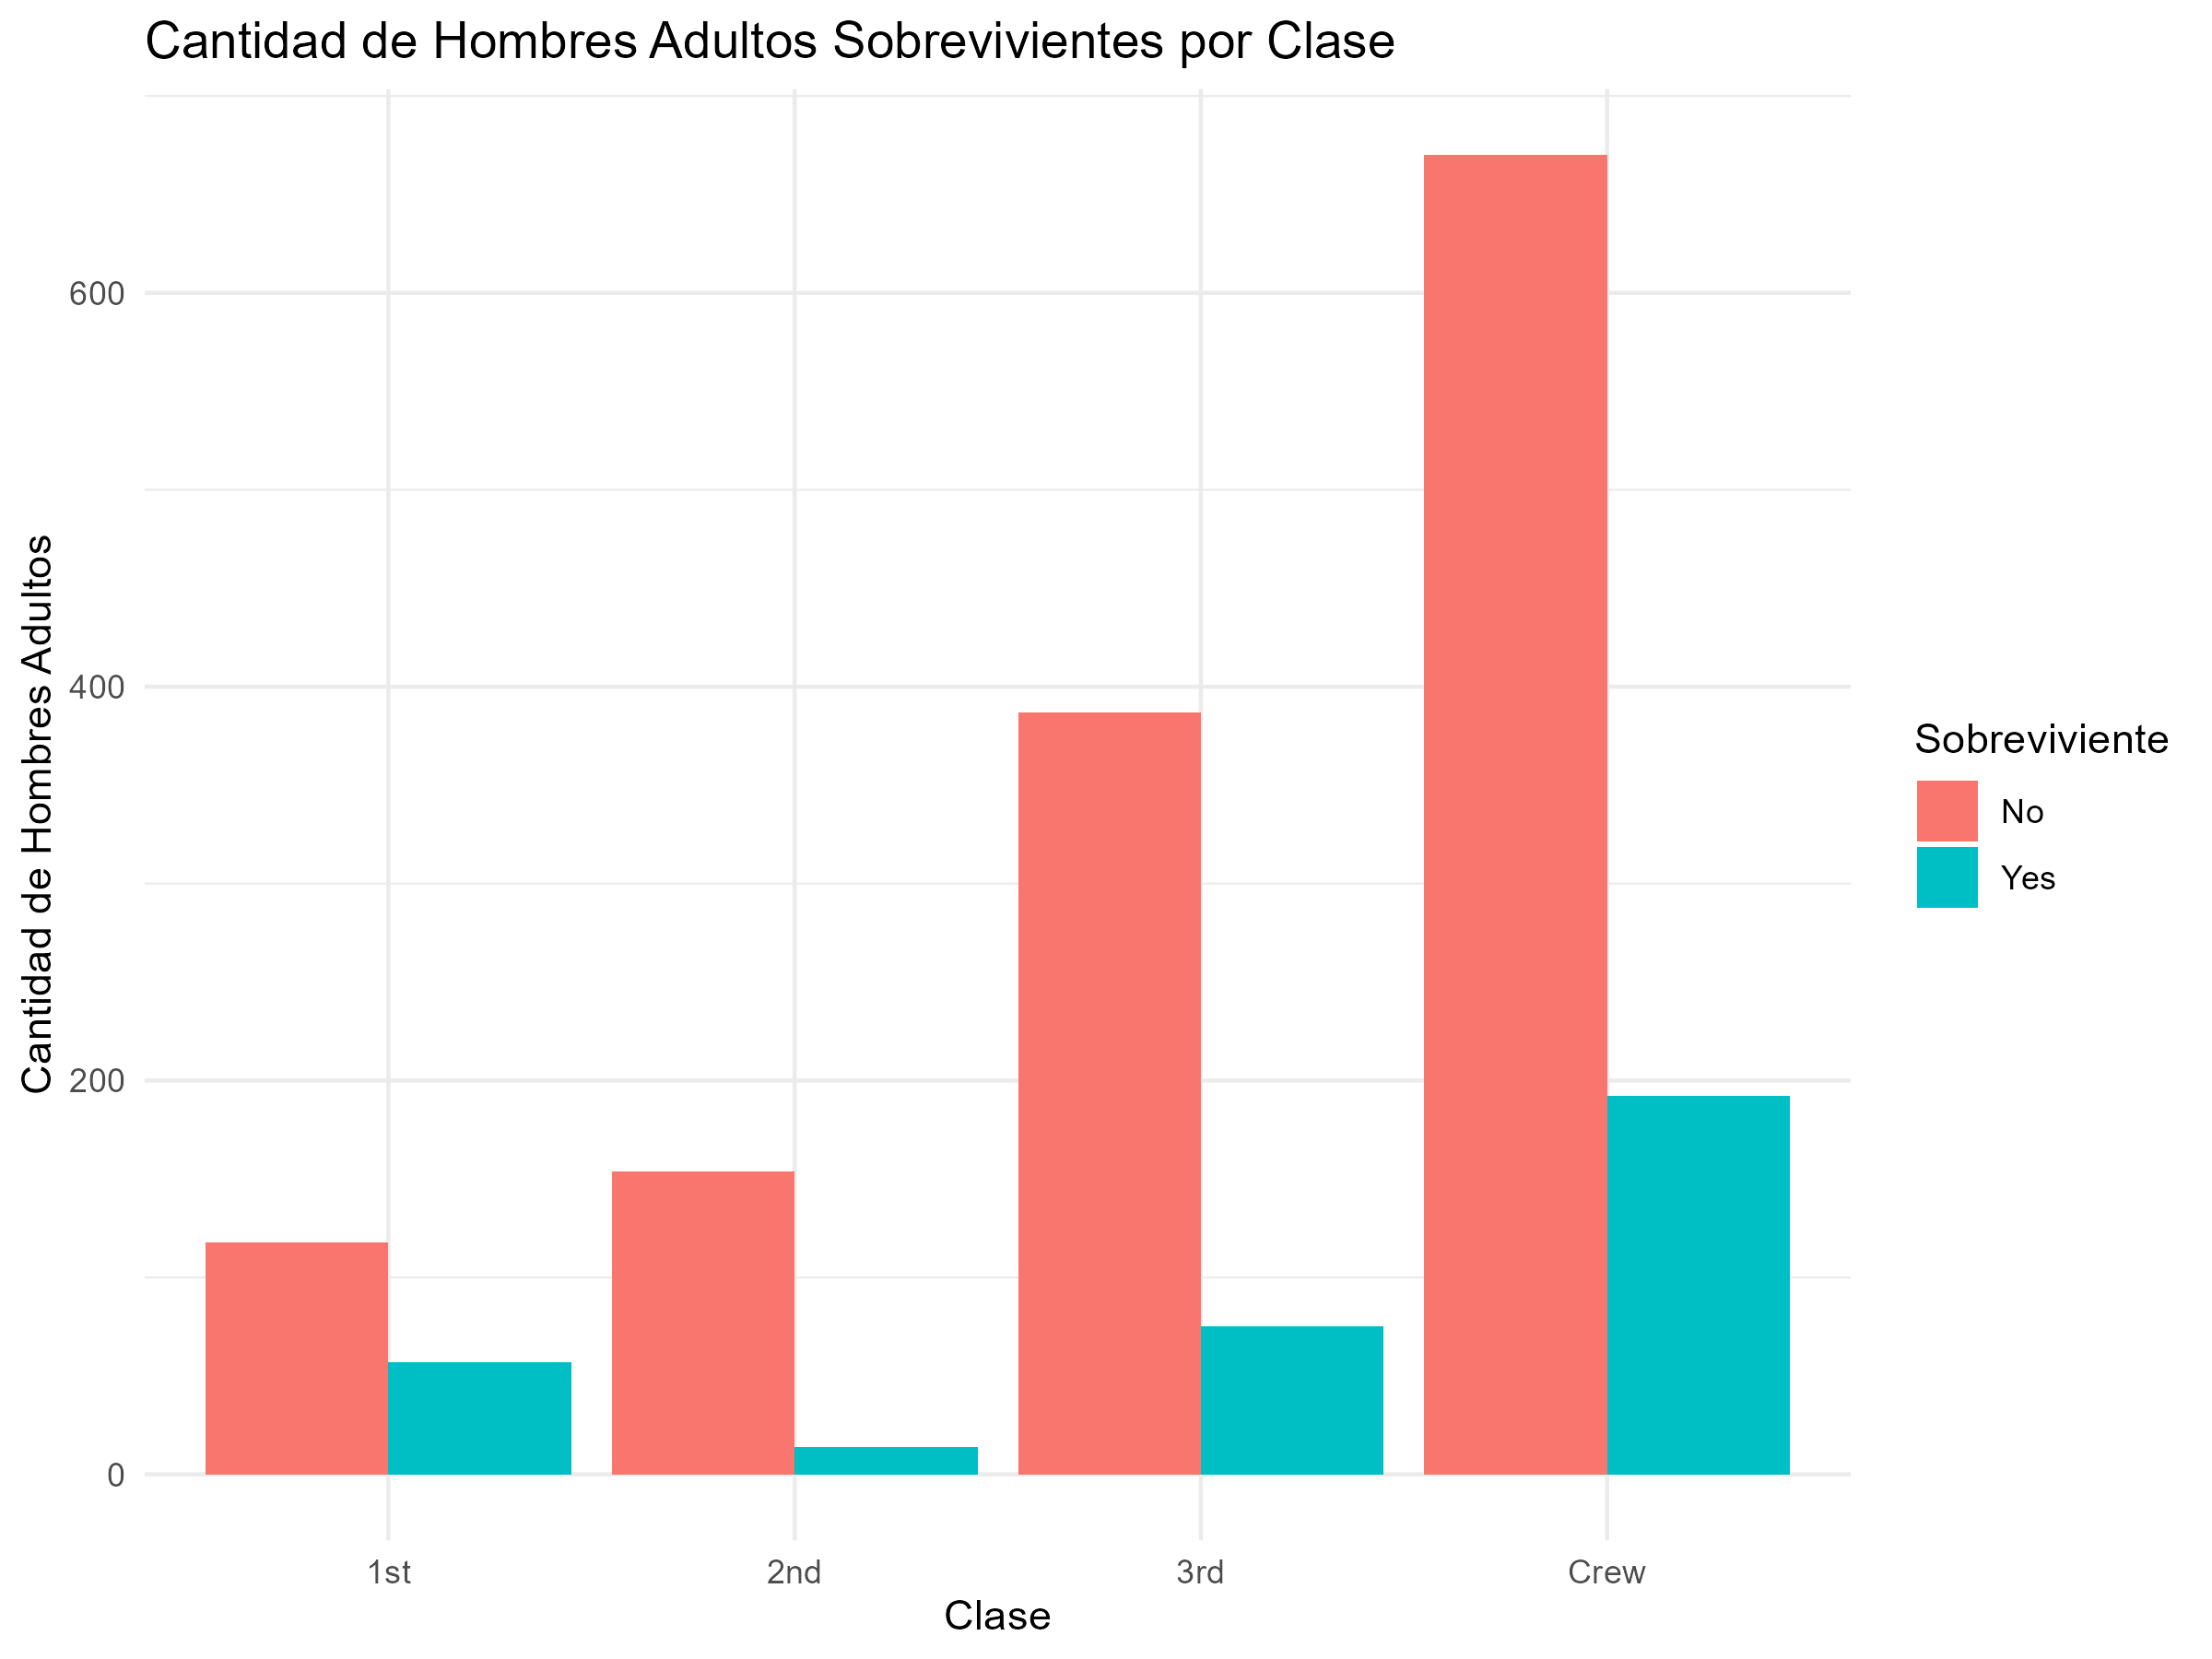
\includegraphics[width=0.8\textwidth]{hombres_adultos_sobrevivientes_por_clase.png}
    \caption{Cantidad de Hombres Adultos Sobrevivientes por Clase}
    \label{fig:hombres_adultos_sobrevivientes_por_clase}
\end{figure}

% Texto adicional o explicación aquí

% Imagen 3: Mujeres Adultas Sobrevivientes por Clase
\begin{figure}[H]
    \centering
    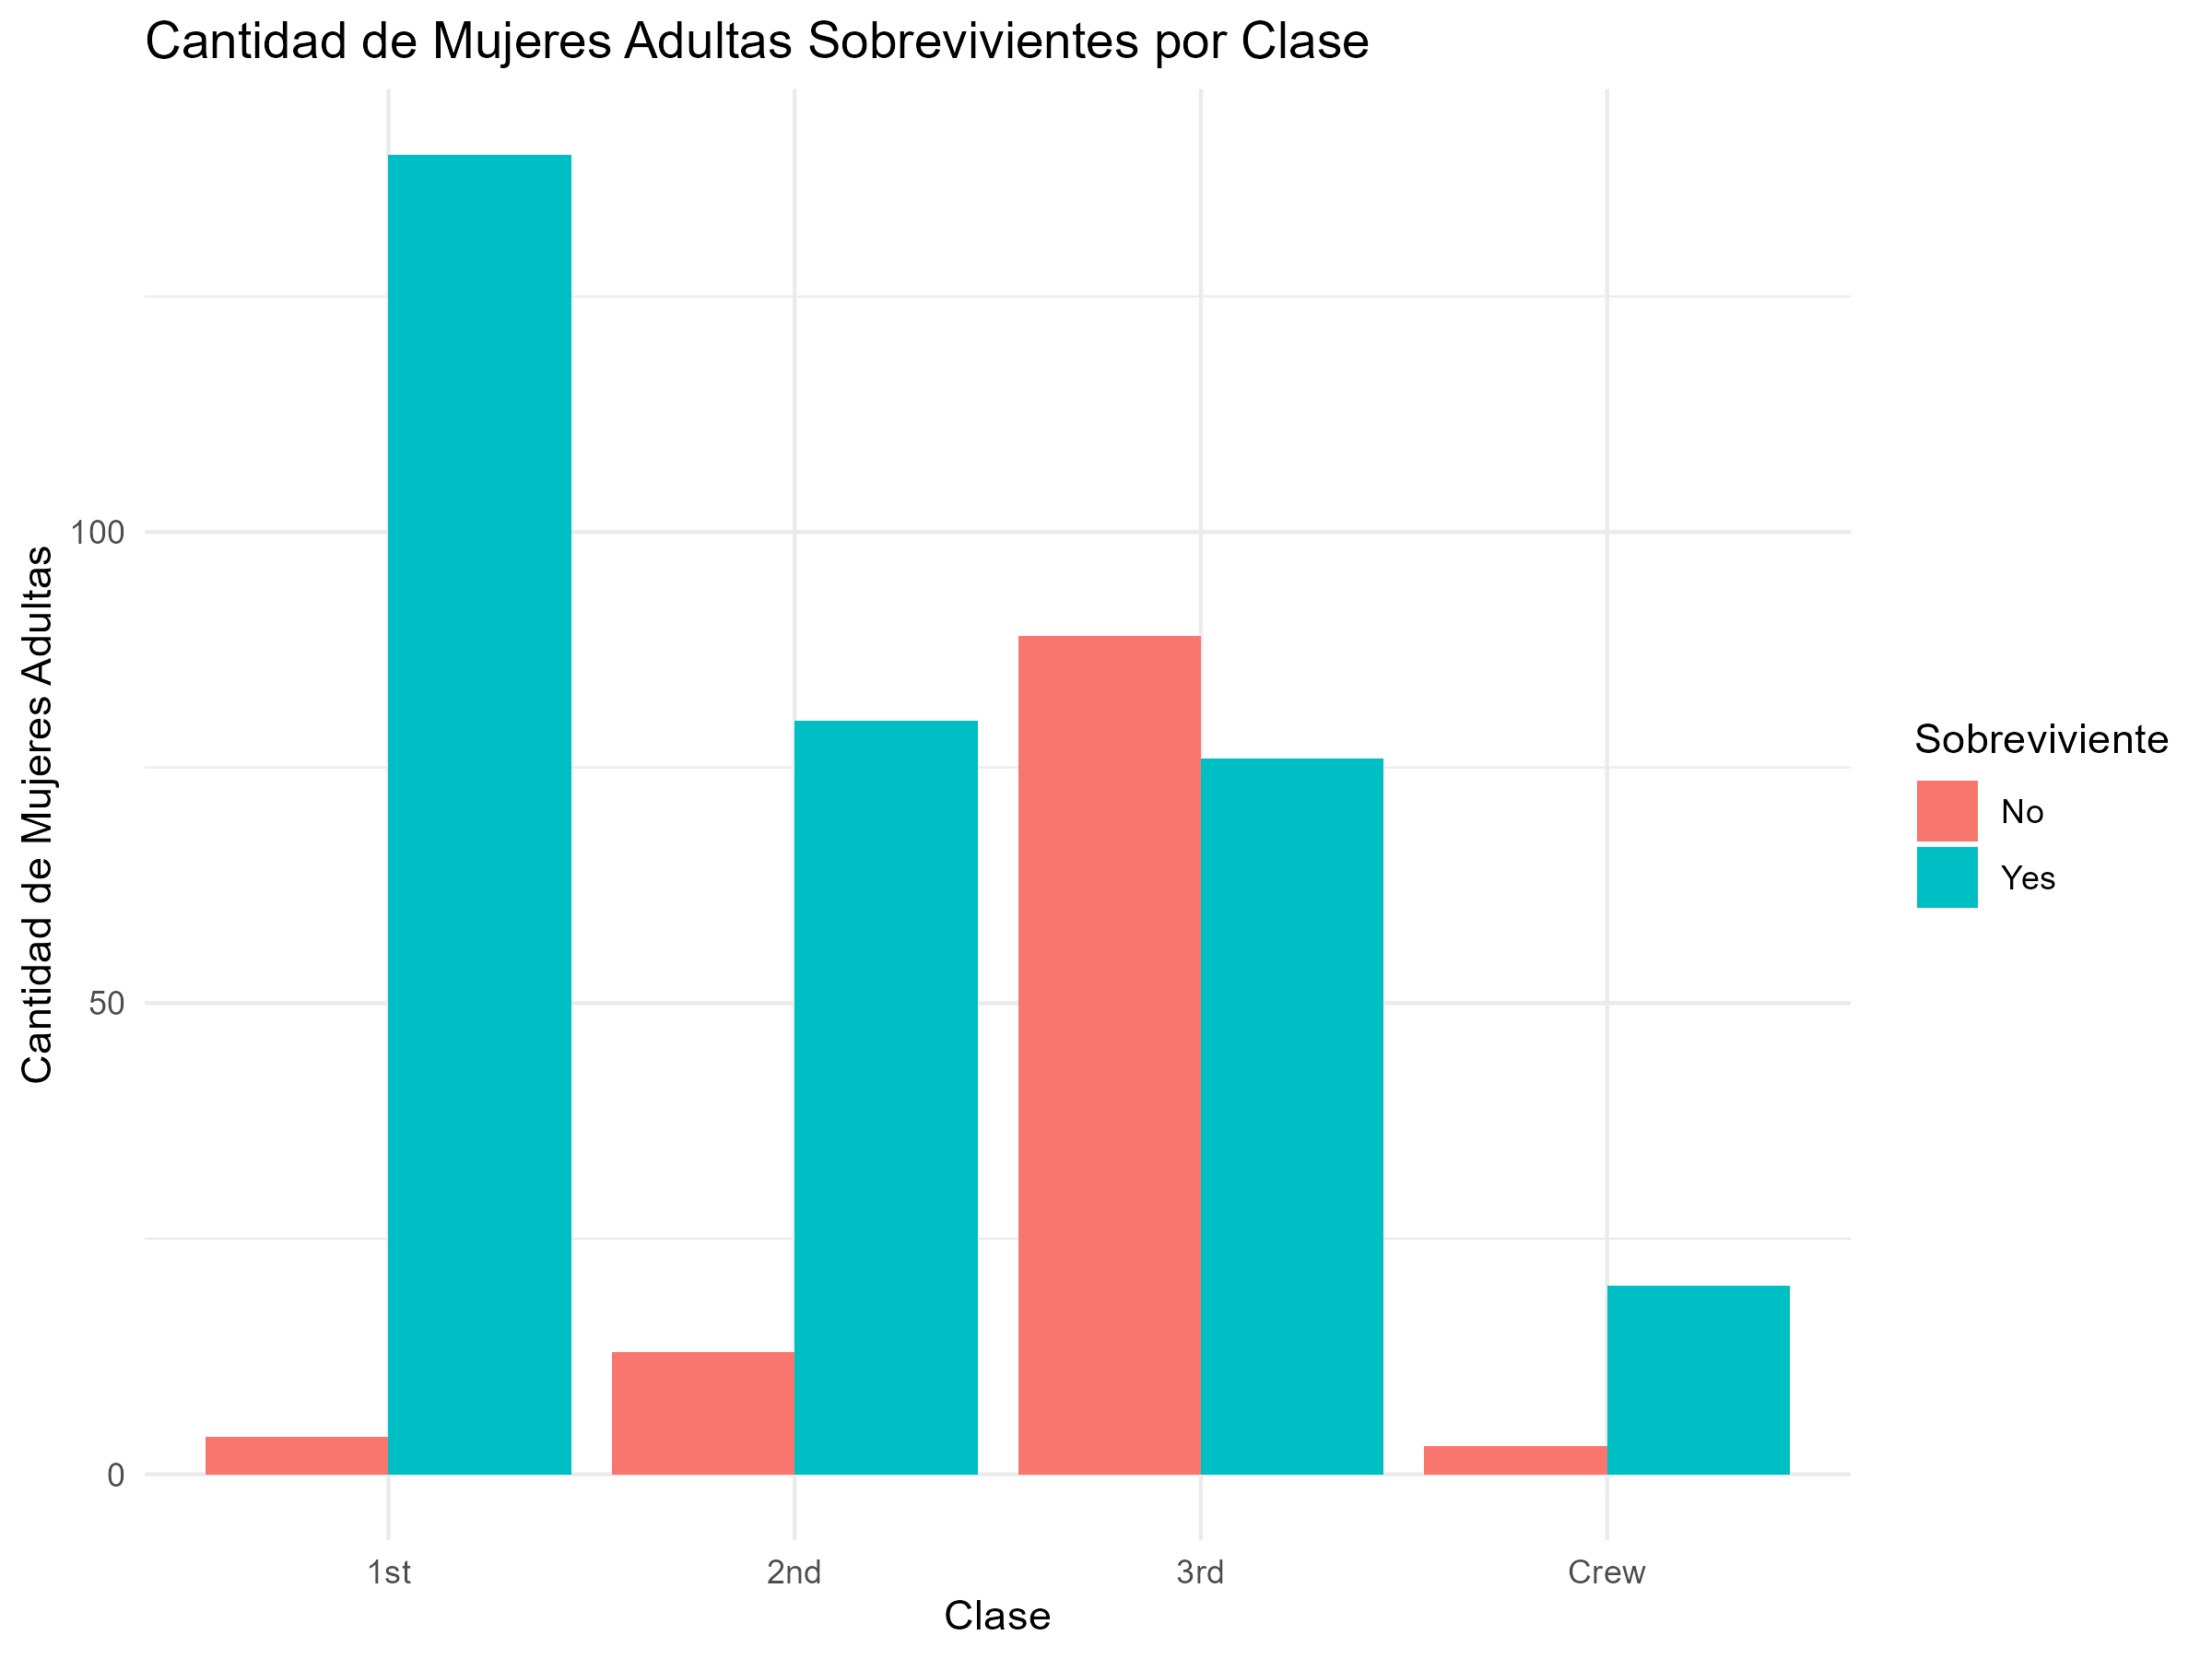
\includegraphics[width=0.8\textwidth]{mujeres_adultas_sobrevivientes_por_clase.png}
    \caption{Cantidad de Mujeres Adultas Sobrevivientes por Clase}
    \label{fig:mujeres_adultas_sobrevivientes_por_clase}
\end{figure}

% Texto adicional o explicación aquí

% Imagen 4: Niñas Sobrevivientes por Clase
\begin{figure}[H]
    \centering
    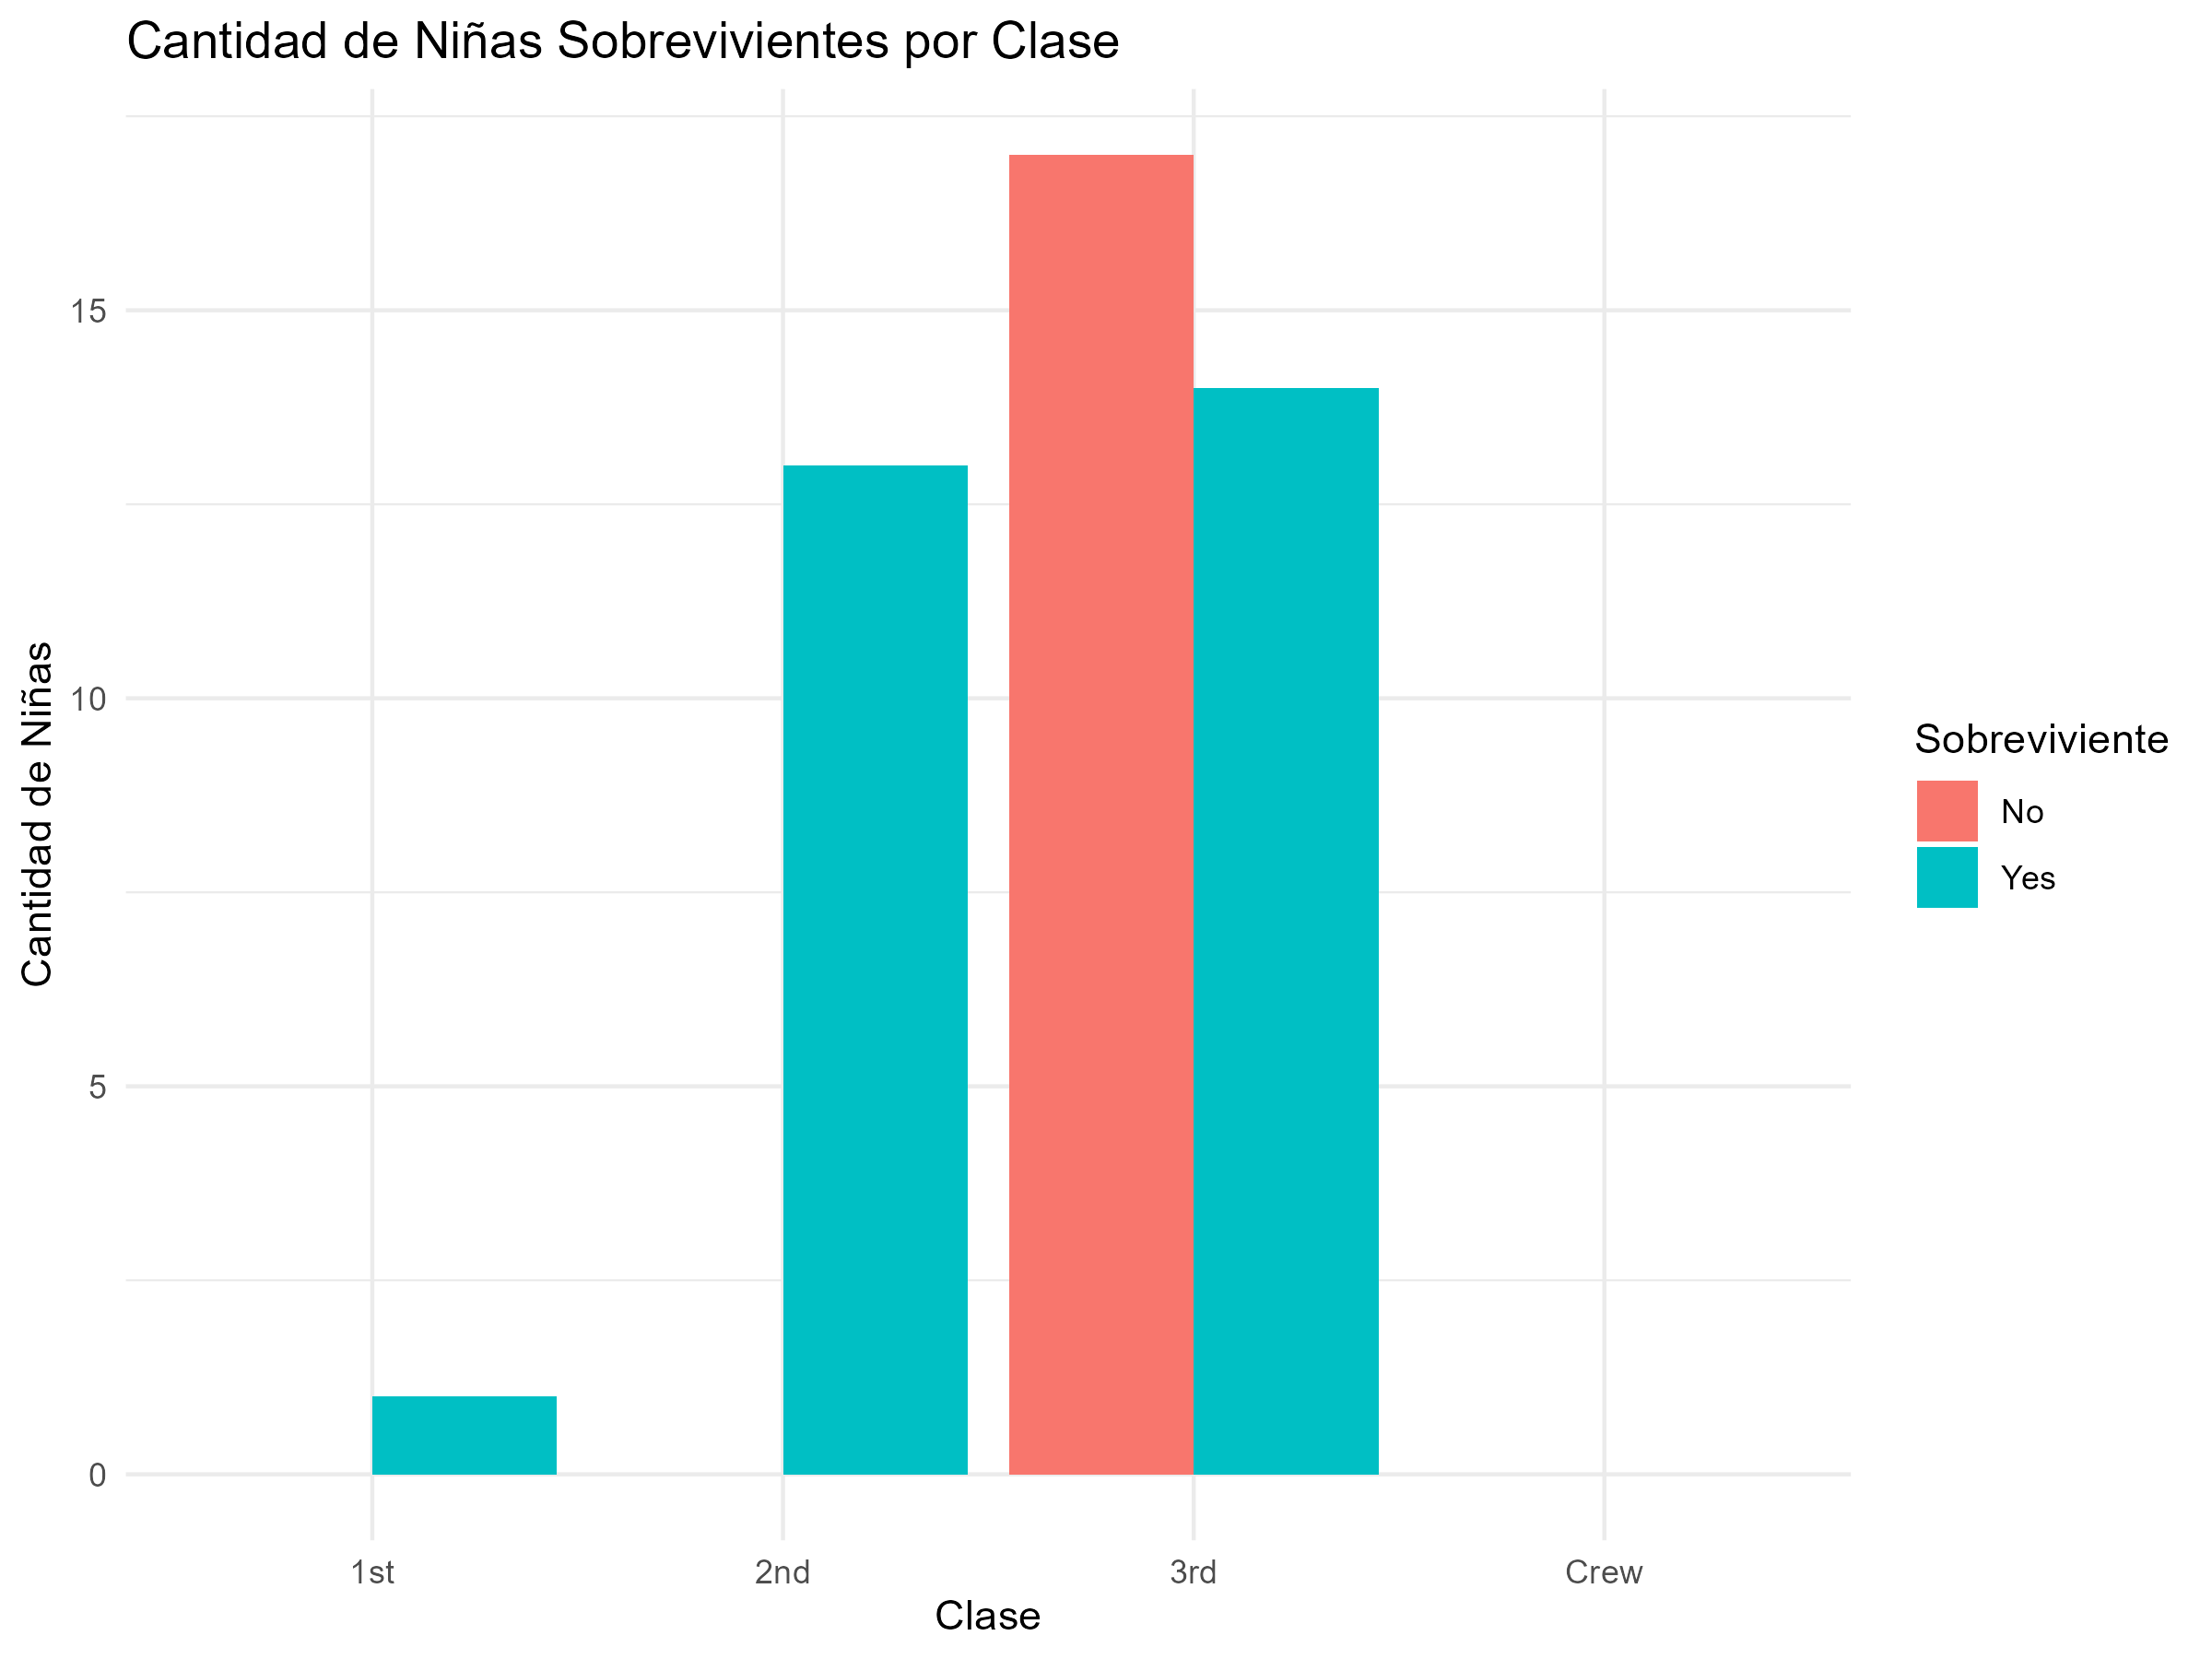
\includegraphics[width=0.8\textwidth]{ninas_sobrevivientes_por_clase.png}
    \caption{Cantidad de Niñas Sobrevivientes por Clase}
    \label{fig:ninas_sobrevivientes_por_clase}
\end{figure}

% Texto adicional o explicación aquí


\end{document}
